

\documentclass{beamer}
\usepackage{graphicx,harvard}
\usetheme{Berlin}

\title{Structure and meaning 2}
\subtitle{What language is}
\author{Liam Keeble}
\institute{School of English Literature, Language and Linguistics}
\date{}

\begin{document}

\frame{\titlepage}

\section{What is language?}

\begin{frame}{A definition}
	\begin{itemize}
	\item The ability to combine smaller units of meaning into larger units of meaning
	\item Only one mechanism: Merge \cite{hauser2002faculty,fitch2004computational}
	
	\end{itemize}
\end{frame}


\begin{frame}{Two definitions}
	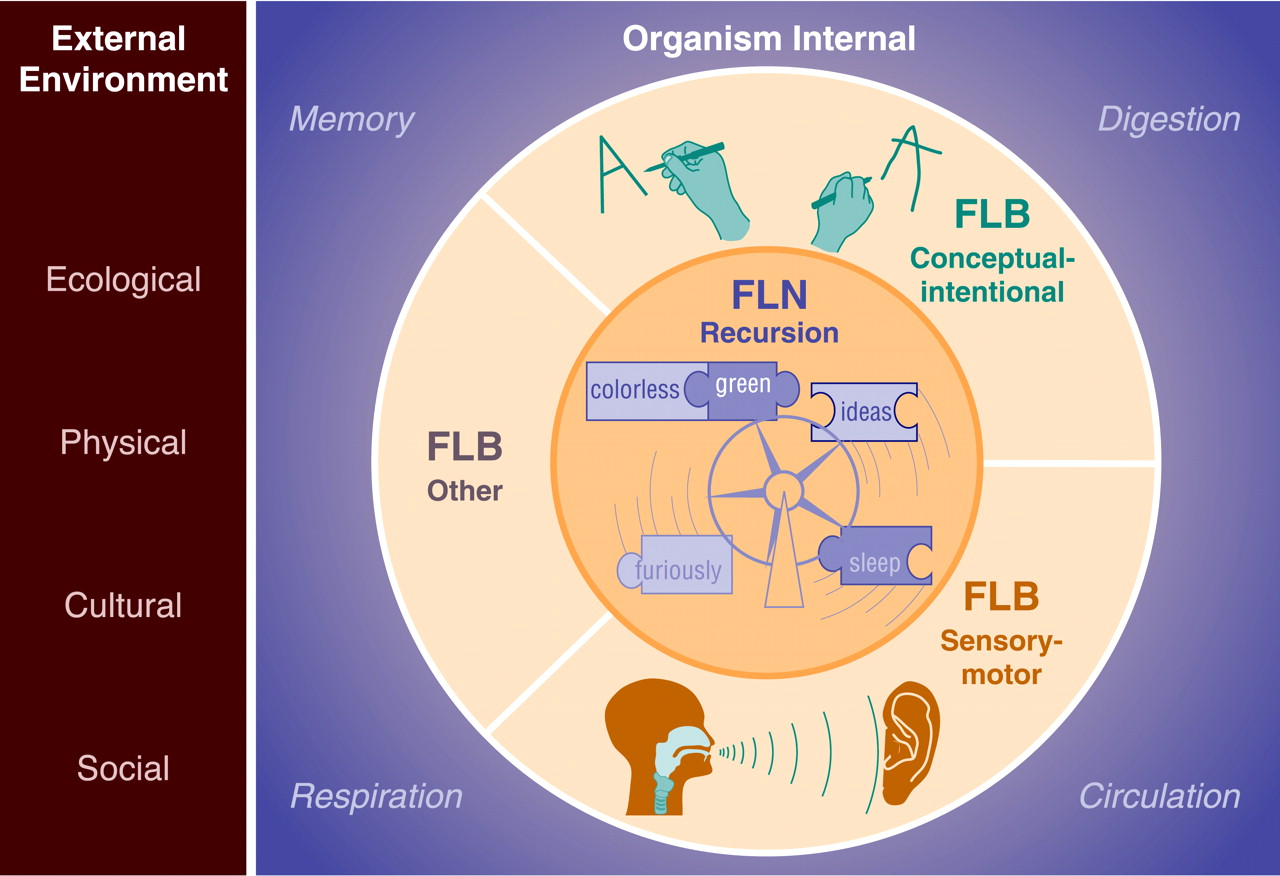
\includegraphics[scale=0.2]{FLN.jpg}
	\nocite{hauser2002faculty}
\end{frame}



\section{How do we communicate?}

\begin{frame}{A definition}
	\begin{itemize}
	\item So maybe we don't use just language when we communicate
	\item But if this is true then where does language fit in to our ability to communicate?
	\item And if we can identify the role of language, then what are the other parts of communication?
	
	\end{itemize}


\end{frame}


\begin{frame}{Shannon model}
	
	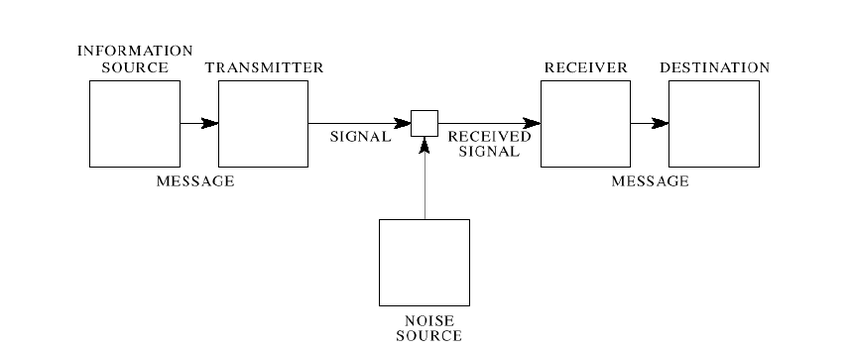
\includegraphics[scale=0.4]{shannon.png}
	\nocite{shannon1948mathematical}
\end{frame}




\section{Language in the brain}

\begin{frame}{Let's focus}
	\begin{itemize}
		\item When we talk about language we talk about something that the human brain can do
		\item A speaker can construct smaller units of meaning into larger units, turn it into sound and send that sound through space
		\item A hearer can then hear that sound and decipher it's linguistic struture to attain something close to the intended meaning of the speaker

	\end{itemize}

\end{frame}


\begin{frame}{The problem of language acquisition}
	\begin{itemize}
	\item 
	\end{itemize}

\end{frame}



\begin{frame}{References}
	\bibliographystyle{agsm}
	\bibliography{references.bib}

\end{frame}


\end{document}


